\documentclass[11pt]{article}
\usepackage[margin=2.7cm]{geometry}
\usepackage{amsmath,amssymb}
\usepackage{graphicx}
\usepackage{url}
\usepackage{array}
\usepackage{xeCJK}
\setCJKmainfont{Hiragino Mincho ProN}
\pagestyle{plain}
\title{太陽近傍の空き度アトラス: 既存不在証拠の異種合算による星単位・技術帯別の占有確率上界台帳 \\[1ex] {\large プレプリント、日本語版。英語版を同一レコードに同梱。\url{doi:10.5281/zenodo.XXXXXXX}}}
\author{前田幸枝(Yukie Maeda) \\ Independent Researcher, Tokyo \\ ORCID: 0009-0005-3401-9230\thanks{AI システムの役割と検証プロトコルの全容は付録 B に開示する。本内部検証は人間による査読の代替ではない。}}
\date{}
\begin{document}
\maketitle

\section*{要旨}

\noindent 太陽近傍の恒星ごとに、「宣言された技術帯 T の設備があれば既存サーベイ集合 S で検出されていたはず」という条件付き不在証拠を合算し、星単位・技術帯別の占有確率上界 P(占有 | D, T, \(\pi\)) を事前確率 \(\pi\) の関数として台帳化した。我々の知る限り、この量の星単位台帳は存在しない。母集団は 100 pc 以内の 332,571 星(Gaia EDR3 GCNS 基盤)\footnote{出所: \texttt{data/phase1/ledger\_v0\_summary.json}(population)。以下、数値の転記元は脚注または表注に示す。再計算は行っていない。}。主張帯は電波 3 帯(T-R1: EIRP \(\geq\) 10\(^{13}\) W、T-R2: \(\geq\) 10\(^{17}\) W、T-R3: 地球級レーダー型間欠漏洩)、[1.10, 3.45] GHz。検出確率は Wlodarczyk-Sroka+20 の 356,616 観測行から取得し、同一モダリティ内の観測は潜在変数で周辺化して併合した。素朴な尤度積が「空き側」に倒れることを定理として示す。閾値・合格基準は合算前に事前登録した(\url{doi:10.5281/zenodo.22067884})。検証: G1 単調性 6,777 検査・違反 0、G2 独立二経路は 4.9 \(\times\) 10\(^{-10}\) dex で一致、G3 は WS20 の 1/N を \(\leq\)50 pc で N = 1513 の完全一致で再現、Hephaistos I 計数は不合格(廃熱帯を降格)、太陽系自己検定は合格。上界を持つ星は T-R1 1,554・T-R2 1,587・T-R3 159、330,984 星(99.52\%)は判定不能であり主結果として報告する。T-R3 では事後 \(\approx\) 事前(\(\Lambda\) \(\geq\) 0.998)であり、空き度を語れる帯の下限は地球自身で校正される。到達可能性・定住資源性との結合では会合到達かつ T-R1 上界を持つ星は 815。DR4(2026-12-02)合流時には距離更新分のみ再計算する(v1.1)。本台帳の上界は測量値であり占有の不在の証明ではなく、入植その他いかなる行為の正当化にも用いない(\S{}7.1)。\par\smallskip


\section*{目次}
\begin{itemize}\setlength{\itemsep}{0pt}
\item[] 要旨
\item[] 1. Introduction
\item[] \hspace{1.2em}1.1 中核の問い
\item[] \hspace{1.2em}1.2 動機
\item[] \hspace{1.2em}1.3 貢献
\item[] \hspace{1.2em}1.4 構成
\item[] 2. Position
\item[] 3. Method
\item[] \hspace{1.2em}3.1 母集団と恒星基盤
\item[] \hspace{1.2em}3.2 技術帯の宣言
\item[] \hspace{1.2em}3.3 検出確率 \(\varepsilon\) の因子構造
\item[] \hspace{1.2em}3.4 併合規則(潜在変数周辺化)と定理
\item[] \hspace{1.2em}3.5 合算式と \(\pi\) 掃引
\item[] \hspace{1.2em}3.6 二段の事前登録
\item[] \hspace{1.2em}3.7 独立性仮定
\item[] \hspace{1.2em}3.8 データ来歴
\item[] 4. Verification
\item[] \hspace{1.2em}4.1 G1: 単調性と MC 安定性
\item[] \hspace{1.2em}4.2 G2: 独立二経路
\item[] \hspace{1.2em}4.3 G3(i): WS20 / Price 系アンカー
\item[] \hspace{1.2em}4.4 G3(ii): Hephaistos I 計数再現(不合格)
\item[] \hspace{1.2em}4.5 G3(iii): 太陽系自己検定(合格)
\item[] \hspace{1.2em}4.6 逸脱節(第9条3項): 制度が機能した二つの実例
\item[] 5. Results
\item[] \hspace{1.2em}5.1 台帳の概観
\item[] \hspace{1.2em}5.2 判定不能 99.52\%: 主結果として
\item[] \hspace{1.2em}5.3 上界曲線
\item[] \hspace{1.2em}5.4 太陽自己校正
\item[] \hspace{1.2em}5.5 W1 情報レイヤ(claim=false)
\item[] 6. Three-axis atlas
\item[] \hspace{1.2em}6.1 結合率
\item[] \hspace{1.2em}6.2 交差計数(合成なし)
\item[] \hspace{1.2em}6.3 定住資源性スライダー
\item[] \hspace{1.2em}6.4 HWC 照合表(合成ではない)
\item[] 7. Discussion
\item[] \hspace{1.2em}7.1 解釈の範囲と限界(Interpretation and scope)
\item[] \hspace{1.2em}7.2 限界と展望(Limitations and outlook)
\item[] 付録 A: \(\varepsilon\) 因子表・受信帯被覆・共通 \(\nu\) グリッド
\item[] 付録 B: Method record and AI disclosure
\item[] 付録 C: 判定不能会計(三軸)
\item[] 付録 D: Reproducibility and data release
\item[] 謝辞
\item[] 参考文献
\end{itemize}
\section*{1. Introduction}

\subsection*{1.1 中核の問い}
\noindent 地球外技術の探索(SETI)は 60 年にわたり不検出を積み上げてきたが、その不検出は「宇宙のどこにも誰もいない」という命題ではなく、「このサーベイが、この感度で、この帯域を、この時刻に見たとき、この星に痕跡はなかった」という星単位・条件付きの事実の集まりである。本稿の問いは、それらの条件付き不在証拠を恒星ごとに異種合算したとき、\textbf{星単位・技術帯別の占有確率上界}がどのように並ぶか、である。この量は、母集団モデルに基づく上限(Grimaldi 系)やサーベイ空間体積の被覆率(Wright+18 のヘイスタック)とは異なり、我々の知る限りこれまで台帳化されていない。\par\smallskip

\subsection*{1.2 動機}
\noindent 本研究の動機は二つである。第一に、人類の生息域拡張を「侵略」ではなく「空いているところを探す」という形で考えるための基礎測量を与えること。第二に、宇宙における技術の稀少性という謎に、星単位の証拠台帳という形で寄与すること。本稿ではこの倫理的要請を方法論に昇格させた。すなわち、すべての言明を「T 帯の設備に関して、サーベイ集合 S のもとで」という条件節を伴う確率文として書き、絶対的な「空いている」を主張しない(\S{}7.1)。\par\smallskip

\subsection*{1.3 貢献}
\noindent (i) 332,571 星の星単位・帯別の \(\varepsilon\)・\(\Lambda\) 台帳(来歴付き)。(ii) 同一モダリティ内の不在証拠を周辺化で併合する規則と、素朴積が空き側に倒れることの定理(\S{}3.4)。(iii) 二段の事前登録(因子構造 \(\rightarrow\) 閾値・合格基準)と逸脱の公開記録。(iv) 判定不能会計を主結果として読む規律。(v) 到達可能性・定住資源性との交差表示(合成なし)。\par\smallskip

\subsection*{1.4 構成}
\noindent \S{}2 位置づけ、\S{}3 方法、\S{}4 検証(逸脱節を含む)、\S{}5 結果、\S{}6 三軸アトラス、\S{}7 Discussion(7.1 解釈の範囲と限界、7.2 限界と展望)。付録 A–D。\par\smallskip

\section*{2. Position}

\noindent \textbf{Grimaldi 系(確率論的母集団モデル)に対して}: Grimaldi (2017) 等は送信機の空間分布・寿命の確率モデルから検出率の期待値を導く。本作は星 i ごとの尤度比 \(\Lambda\)\_i(T) を台帳化し、母集団の仮定を置かない(\(\pi\) は掃引する)。\par\smallskip
\noindent \textbf{Wright+18 ヘイスタックに対して}: Wright, Kanodia \& Lubar (2018) は探索パラメータ空間の体積被覆率を論じる。本作はその射影を個別星に落とし、被覆の穴を「判定不能」として星単位で計数する。判定不能 99.52\%(\S{}5.2)はヘイスタック不完備性の星単位版である。\par\smallskip
\noindent \textbf{Breakthrough Listen・\^{G}/Hephaistos に対して}: Price+20・Wlodarczyk-Sroka+20(以下 WS20)は新規電波観測と母集団上限、Wright+14/Griffith+15 と Suazo+22/24 は中赤外廃熱の探索である。本作は新規観測を行わず、これらの\textbf{既存不在証拠を星単位で異種合算}する。Phase 0 の実査で、\^{G} には近傍恒星の個別上限が存在せず(銀河対象)、Hephaistos は方法が公刊文献で閉じるが星単位表は非公開であることを確認した\footnote{\texttt{docs/phase0/01-machine-readability-survey.md}。}。\par\smallskip
\noindent \textbf{上限算式の多様性}: Price+20 \S{}5.3 の百分率上限(算式非明記)、WS20 の 1/N、本作の二項厳密上限と星単位ベイズ上界は、いずれも\textbf{別量}である(\S{}4.3、\S{}7.1)。\par\smallskip


\section*{3. Method}

\subsection*{3.1 母集団と恒星基盤}
\noindent GCNS(Gaia Collaboration, Smart et al. 2021; VizieR J/A+A/649/A6)の 331,312 星(\(\leq\)100 pc)と、同カタログの \texttt{missing} 表(EDR3 に解が無い明るい星)1,259 星、計 332,571 星\footnote{出所: \texttt{data/phase1/ledger\_v0\_summary.json}(population)。以下、数値の転記元は脚注または表注に示す。再計算は行っていない。}。EDR3 の source\_id は DR3 と同一である。距離は GCNS の dist\_50。WS20 の星(Gaia DR2 ID)は位置・固有運動で EDR3 に照合した(\(\leq\)100 pc で 1,534/1,671 = 91.8\%。残りは主に EDR3 に解の無い明るい星で、\texttt{missing} 表により 67 観測行・42 星を回収した。Phase 0 の実査値 43 は DR2 単位の計数で、HD 239960A に DR2 2 星が対応するため 42 エントリとなる)\footnote{\texttt{data/phase0/gcns\_stats.json}、\texttt{data/phase1/ledger\_v0\_summary.json}(n\_rows\_matched\_missing\_table)。}。\par\smallskip


\subsection*{3.2 技術帯の宣言}
\noindent 技術帯 T は宣言されたクラスの有限集合である(憲法第3条1項)。\par\smallskip
\begin{itemize}\setlength{\itemsep}{1pt}
\item \textbf{T-R1}: 狭帯域(\(\delta\)\(\nu\) = 1 Hz)・連続送信、EIRP \(\geq\) 10\(^{13}\) W(Arecibo 惑星レーダー級)。送信周波数 \(\nu\) は窓 [1.10, 3.45] GHz 内で一様と宣言(窓内の被覆の穴は \(\varepsilon\)(\(\nu\)) 側で表現)。
\item \textbf{T-R2}: 同上、EIRP \(\geq\) 10\(^{17}\) W。
\item \textbf{T-R3}: 地球級レーダー型間欠漏洩、EIRP\_peak = 10\(^{11}\) W(クラス上端で評価)、照射因子 f\_ill = f\_duty\(\cdot\)f\_beam \(\in\) [10\(^{-5}\), 10\(^{-2}\)](対数一様、星単位の潜在変数として周辺化)。放送型漏洩(\textasciitilde{}10\(^{6}\) W)は帯の下限外。
\item \textbf{T-W1(情報レイヤ)}: 部分ダイソン球型廃熱(\(\gamma\) \(\geq\) 0.1、T\_DS \(\in\) [100, 700] K)。G3(ii) 不合格により v1 では空き度を主張しない(\S{}4.4、\S{}5.5)。
\item 拡張区画(光学レーザー、遷移現象、未公刊の C/X 帯・UWL 観測)は判定不能。
\end{itemize}

\subsection*{3.3 検出確率 \(\varepsilon\) の因子構造}
\noindent 観測 s(望遠鏡 \(\times\) 受信帯 \(\times\) ポインティング)、星 i、帯 T について、\(\varepsilon\)\_\{s,i\}(T; \(\nu\)) = \(\Theta\)\_sens \(\cdot\) 1[\(\nu\) \(\in\) B\_s] \(\cdot\) f\_pipe \(\cdot\) f\_duty \(\cdot\) f\_drift \(\cdot\) f\_beam。\par\smallskip
\begin{itemize}\setlength{\itemsep}{1pt}
\item 感度: \(\Theta\)\_sens = 1[EIRP\_min,s,i \(\leq\) EIRP\_T]、EIRP\_min = EIRP50 (d/50 pc)\(^{2}\) / R(\(\theta\))、EIRP50 = 2.1 \(\times\) 10\(^{12}\) W(GBT L/S)、9.1 \(\times\) 10\(^{12}\) W(Parkes 10-cm)(Price+20 \S{}5.2)、R(\(\theta\)) = exp(\(-\)4 ln 2 (\(\theta\)/FWHM)\(^{2}\))(WS20 \S{}3)。WS20 表の全 356,616 行をこの式で再計算し、比の中央値は 1.0000 であった\footnote{\texttt{data/phase0/ws20\_stats.json}(eirp\_recalc\_check)。}。クラスの最弱成員(閾値ちょうど)で評価する(保守側)。
\item 帯域被覆: B\_s は受信帯からノッチを除いた区間(GBT L 0.66 GHz、GBT S 0.94 GHz、Parkes 10-cm 0.85 GHz、合成 2.15 GHz / 窓 2.35 GHz)。
\item f\_pipe = 0.5(Price+20 \S{}5.3 の 1 観測あたり検出確率。RFI 遮蔽込み)。f\_duty = f\_drift = f\_beam = 1(T-R1/R2 のクラス宣言)。
\item T-W1: Hephaistos 式モデル(灰色吸収 (1\(-\)\(\gamma\))、黒体再放射)で G\(-\)W3 / G\(-\)W4 の色超過を予測し、主系列軌跡から k = 3 \(\sigma\) の超過で検出。既超過星は「検出候補」として判定不能。
\end{itemize}


\subsection*{3.4 併合規則(潜在変数周辺化)と定理}
\noindent 同一モダリティ内の観測は、共有される潜在変数(電波: \(\nu\)、間欠帯: f\_ill、廃熱: T\_DS)で周辺化して一本の \(\varepsilon\) に併合し、モダリティ間でのみ積をとる:\par\smallskip

\noindent   1 \(-\) \(\varepsilon\)\(^{\mathrm{rad}}\)\_i(T) = \(\Sigma\)\_c w\_c \(\Pi\)\_\{s\(\in\)rad(i)\} [1 \(-\) \(\varepsilon\)\_\{s,i\}(T)\(\cdot\)1[c \(\subset\) B\_s]]、 T-R3: 1 \(-\) \(\varepsilon\)\(^{\mathrm{rad}}\)\_i = \(\Sigma\)\_f w\_f \(\Sigma\)\_c w\_c \(\Pi\)\_s [1 \(-\) \(\Theta\)\_s f\_pipe f\(\cdot\)1[c \(\subset\) B\_s]]\par\smallskip

\noindent ここで c は窓を受信帯境界・ノッチ境界で分割した 9 区間(モダリティ全体で共通のグリッド)、w\_c は幅の比、f は 13 点対数格子。\par\smallskip

\noindent \textbf{定理(素朴積の空き側バイアス)}。\textbf{前提}: (a) 送信周波数 \(\nu\) は全観測に共通の未知量で、窓内一様事前をもつ; (b) 同一受信帯の観測は同じ被覆区間 B をもち、帯内の検出確率 p は観測ごとに等しく、帯外では 0; (c) 観測は \(\nu\) を与えたとき条件付き独立。このとき同一帯 2 回観測の厳密な非検出確率(= \(\Lambda\))は 1 \(-\) c(1 \(-\) (1\(-\)p)\(^{2}\)) = 1 \(-\) c(2p \(-\) p\(^{2}\))(c = |B|/|窓|)、素朴積は (1 \(-\) cp)\(^{2}\) であり、0 < c < 1、0 < p \(\leq\) 1 で \textbf{(1 \(-\) cp)\(^{2}\) < 1 \(-\) c(2p \(-\) p\(^{2}\))} が成立する。p = 1 では厳密 1 \(-\) c に対し素朴積 (1\(-\)c)\(^{2}\)。\textbf{証明}: 差 [1 \(-\) c(2p \(-\) p\(^{2}\))] \(-\) (1\(-\)cp)\(^{2}\) = c p\(^{2}\) (1 \(-\) c) > 0。\(\blacksquare\) 素朴積は非検出確率 \(\Lambda\) を小さく(検出確率を大きく)評価し、事後占有確率 expit(logit \(\pi\) + ln \(\Lambda\)) を低く、すなわち「空き側」に倒す。単体テスト \texttt{test\_merge\_rule\_same\_band\_twice} でこの不等式を固定している。同様に f\_ill を観測行ごとに独立に引くことは f\_beam(送信機側の幾何)が観測者方向に固定されている事実に反し、同方向の誤りを生む。f\_ill の全共有は保守的宣言である(真の構造は f\_beam 共有・f\_duty 部分独立の中間にあり、Jensen の不等式より全共有は \(\varepsilon\) を下界側に置く。すなわち検出力を過小申告する側であり、占有を除外できない方向に倒れる)。\par\smallskip

\subsection*{3.5 合算式と \(\pi\) 掃引}
\noindent \(\Lambda\)\_i(T) = 1 \(-\) \(\varepsilon\)\(^{\mathrm{m}}\)\_i(T)(v1 では各帯は単一モダリティ)。P(占有 | D, T, \(\pi\)) = expit(logit \(\pi\) + ln \(\Lambda\)\_i(T))。\(\pi\) は [10\(^{-6}\), 0.5] の対数 51 点で掃引し、代表 \(\pi\) = 10\(^{-3}\), 10\(^{-2}\), 10\(^{-1}\) を併記する。単一の数値を「空き度」と呼ばない。計算は対数空間(logsumexp)で行う。\par\smallskip

\subsection*{3.6 二段の事前登録}
\noindent (a) Phase 0 末: 技術帯集合・\(\varepsilon\) の因子構造・併合規則をコミット \texttt{10a01e71…}(付録 D)で固定(非公開)。(b) Phase 1 末: 具体閾値・合算式・G1–G3 合格基準・MC 宣言を Zenodo に公開登録(\url{doi:10.5281/zenodo.22067884}、sha256 88eb7809\ldots{})し、その後に合算を走らせた。以後の変更は逸脱として \S{}4.6 に記載する。\par\smallskip

\subsection*{3.7 独立性仮定}
\noindent 併合後に残る仮定を宣言する: f\_pipe の観測間独立(Price+20 と同一前提、感度枠 U[0.3, 0.8])、稼働率の時間独立(T-R1/R2 は連続送信クラス)、T-R3 照射因子の星単位共有、距離の星単位共有、W3/W4 判定の OR 併合、主系列軌跡の経験的構築、DS 黒体流束の単色近似(\(\pm\)10\%)。\par\smallskip

\subsection*{3.8 データ来歴}
\noindent WS20 表(VizieR J/MNRAS/498/5720、356,616 行)\footnote{\texttt{data/phase0/ws20\_stats.json}(eirp\_recalc\_check)。}、Breakthrough Listen 公開アーカイブ(目標別観測ファイル: HIP 目標 6,219 件、観測日・中心周波数 100\%、観測ファイル 95,529 件; 電波観測行 2,259 のうち 1,934 行に観測日 MJD を付与)\footnote{\texttt{data/phase0/bl\_log\_stats.json}、\texttt{data/phase1/ledger\_v0\_summary.json}(rows\_with\_bl\_dates)。}、GCNS、HGCA(Hipparcos–Gaia 照合、BL 目標 6,219 \(\rightarrow\) DR3 5,963)、Mamajek 表(M\_G \(\rightarrow\) logL、色 \(\rightarrow\) 型)、NASA Exoplanet Archive(pscomppars、2026-08-23 取得)、HWC(2026-08-23 取得)。全入力の sha256 は付録 D。\par\smallskip


\section*{4. Verification}

\subsection*{4.1 G1: 単調性と MC 安定性}
\noindent 観測行を 1 つずつ加えた \(\Lambda\) の列が非増加であることを全星(1,587)\(\times\) 3 帯で検査した: \textbf{6,777 検査、違反 0}(許容 +10\(^{-12}\))\footnote{\texttt{data/phase2/g1\_report.json}。}。MC(N = 1,000、seed = 20260823、共有単位は事前登録 \S{}4 どおり)では、電波帯の log\(_{10}\)\(\Lambda\) の 90\% 区間幅の中央値は 0.094 dex(f\_pipe の摂動が支配、観測行数に比例)、低信頼セル(幅 > 0.5 dex)は電波 3 帯で 0。情報レイヤ W1 では低信頼 25,822(\(\gamma\) = 0.1)だが、その 97\% は \(\Lambda\) = 0(クリップ)と小さな正値の間の離散的な跳びに由来し、事後 @\(\pi\) = 10\(^{-2}\) で見れば「占有確率 \(\lesssim\) 10\(^{-3}\)」の結論は不変である。\par\smallskip


\subsection*{4.2 G2: 独立二経路}
\noindent \(\Lambda\) 列を含まないエクスポート(星 \(\times\) 帯 \(\times\) 区間の \(\varepsilon\) 行・区間重み)を合算前に参謀(チャット Claude)に渡し、参謀が対数和で \(\Lambda\) を独立再計算した。突合結果は max|\(\Delta\)log\(_{10}\)\(\Lambda\)| = 4.9 \(\times\) 10\(^{-10}\)(電波)、5.2 \(\times\) 10\(^{-7}\)(廃熱)、許容 10\(^{-6}\)、違反 0\footnote{裁定ログ「G2 合格」。}。\par\smallskip


\subsection*{4.3 G3(i): WS20 / Price 系アンカー}
\noindent (a) \textbf{報告(合否なし)}: Price+20 \S{}5.3 の公刊値 0.45\% / 0.37\% / 2.0\%(GBT L / GBT S / Parkes、N = 882 / 1005 / 189)に対し、当方の二項厳密 95\% 上限 f = [1 \(-\) 0.05\(^{1/N}\)] / 0.5 は 0.678\% / 0.595\% / 3.15\%(比 1.51 / 1.61 / 1.57)。原典の算式は本文に明記されておらず、公刊三値から逆算した f\(\cdot\)N = 3.97 / 3.72 / 3.78 はばらつき、単一の標準式では同時再現できない\footnote{\texttt{data/phase3/g3\_report.json}。}。\par\smallskip
\noindent (b) \textbf{ハードゲート}: WS20 表の \texttt{rest} 距離(DR2 基盤)のみで再計数した(EDR3 距離は不使用)。公刊の「EIRP \(\gtrsim\) 6.5 \(\times\) 10\(^{13}\) / 2.5 \(\times\) 10\(^{14}\) W」は殻内 EIRP\_min の最大値(再計数 6.49 \(\times\) 10\(^{13}\) / 2.49 \(\times\) 10\(^{14}\) W)であり、絞り込み条件ではない。\(\leq\)50 pc: \textbf{N = 1513(完全一致)}、1/N = 0.0661\%(公刊 \(\lesssim\)0.0660\%); \(\leq\)100 pc: N = 1671、0.0598\%(公刊 0.061 +0.001/\(-\)0.003 \%); \(\leq\)200 pc: N = 2576、0.0388\%(公刊 0.039 +0.004/\(-\)0.008 \%)。\(\leq\)100/200 pc は公刊の明示誤差区間の内側にある(合格基準は \S{}4.6 の逸脱による)。\par\smallskip
\noindent (c) \textbf{別量}: 同じ殻の本作の星単位事後の平均は、\(\pi\) = 10\(^{-3}\) / 10\(^{-2}\) で 7.7 \(\times\) 10\(^{-4}\) / 7.7 \(\times\) 10\(^{-3}\)(mean \(\Lambda\) \(\approx\) 0.767、\(\leq\)50 pc、ok 1,436 星)。1/N は「N 回の不検出試行」の頻度論上限で被覆率・感度因子を含まず、本作の事後平均は \(\pi\) の関数である。\(\pi\) = 10\(^{-3}\) で同桁になるのは \(\Lambda\) \(\approx\) 0.77 が 1 に近いことの帰結であり、一致ではない。\par\smallskip


\subsection*{4.4 G3(ii): Hephaistos I 計数再現(不合格)}
\noindent Suazo+22 Table 1(100 pc、N = 265,724、T\_DS = 300 K)の「DS 適合(排除できない)率」6.6 \(\times\) 10\(^{-3}\) / 1.9 \(\times\) 10\(^{-4}\) / 1.8 \(\times\) 10\(^{-5}\)(\(\gamma\) = 0.1 / 0.5 / 0.9)を、本作の母集団(GCNS \(\leq\)100 pc 300,567 \(\rightarrow\) 主系列 276,814 \(\rightarrow\) WISE 測光あり 187,274)と超過判定で計数した。適合 = 「300 K 区間で \(\theta\)\(_{3}\) = \(\theta\)\(_{4}\) = 0」または「既超過の検出候補」(定義 A)とすると、適合率は 2.07 \(\times\) 10\(^{-2}\) / 1.77 \(\times\) 10\(^{-2}\) / 1.77 \(\times\) 10\(^{-2}\)、比は \textbf{3.13 / 93 / 982} で凍結基準(比 0.3–3)を外れ、\textbf{不合格}である\footnote{\texttt{data/phase3/g3\_report.json}。}。\par\smallskip
\noindent \textbf{方向分析(計算誤りではない)}: 比が \(\gamma\) とともに爆発する構造は、本作の「検出候補」(\(\geq\)3\(\sigma\) 超過、3,304 星)が第5条3項により\textbf{全 \(\gamma\) で「排除できない」側に置かれる}ことに由来する。Hephaistos の「DS 領域内」は (\(\gamma\), T) ごとのモデル領域への所属で、0.2 等級の軽い超過は \(\gamma\) = 0.9(数等級)と整合しない。本作は Hephaistos より除外を少なく主張する保守設計の帰結であり、計算誤りではない(G1・G2 は W1 でも合格している)。\par\smallskip
\noindent \textbf{定義 B の診断}(採用せず): 観測残差が (\(\gamma\), 300 K) モデル残差と k\(\sigma\)\_tot 以内で整合する星を適合とすると、比は \(\gamma\) = 0.1 で 0.82、\(\gamma\) = 0.5 で 0.17(6 星 vs 期待 \textasciitilde{}36 星、ポアソンで説明不能・未解明)、\(\gamma\) = 0.9 で 0.30(\textasciitilde{}1 vs \textasciitilde{}3.4 星、小数統計で判定不能)。数字を見た後の適合定義の選択にあたるため採用せず、合格を示唆する語は用いない。\par\smallskip
\noindent \textbf{帰結}: 憲法第6条(本作導出の帯は対応する G3 アンカー合格を公開の前提条件とする)により、T-W1 を拡張区画(情報レイヤ、claim=false)へ降格した。\par\smallskip
\noindent \textbf{昇格経路}: Hephaistos 系の星単位表が公開された場合、または DR4 合流(v1.1)で独立アンカーが組めた場合に再判定する(こちらから提供依頼は行わない)。\par\smallskip

\subsection*{4.5 G3(iii): 太陽系自己検定(合格)}
\noindent 太陽系を d = 1.3–10.8 pc の 24 点(GBT L + GBT S + Parkes 10-cm、軸上、各 1 観測行、EIRP\_peak = 10\(^{11}\) W)の仮想行として T-R3 に通した。全 d で \(\Lambda\)(周辺化) \(\geq\) 0.999085、\(\Lambda\)(f\_ill 上端 10\(^{-2}\)) \(\geq\) 0.99479、すなわち\textbf{事後 \(\approx\) 事前}であり合格\footnote{\texttt{data/phase3/g3\_report.json}。}。赤信号の動作確認: f\_ill = f\_pipe = 1 の極では \(\Lambda\) = 1 \(-\) 2.15/2.35 = 0.0851 < 0.5(d \(\leq\) 4.8 pc で 3 帯とも感度内)となり地球は「検出される」。\(\varepsilon\)(検出器)は生きており、T-R3 で事後 \(\approx\) 事前になるのは照射因子(間欠・指向)が小さいためである。Parkes 10-cm は d > 5.24 pc で感度外、GBT は 10.9 pc まで(図 1)。\par\smallskip

\begin{figure}[t]\centering
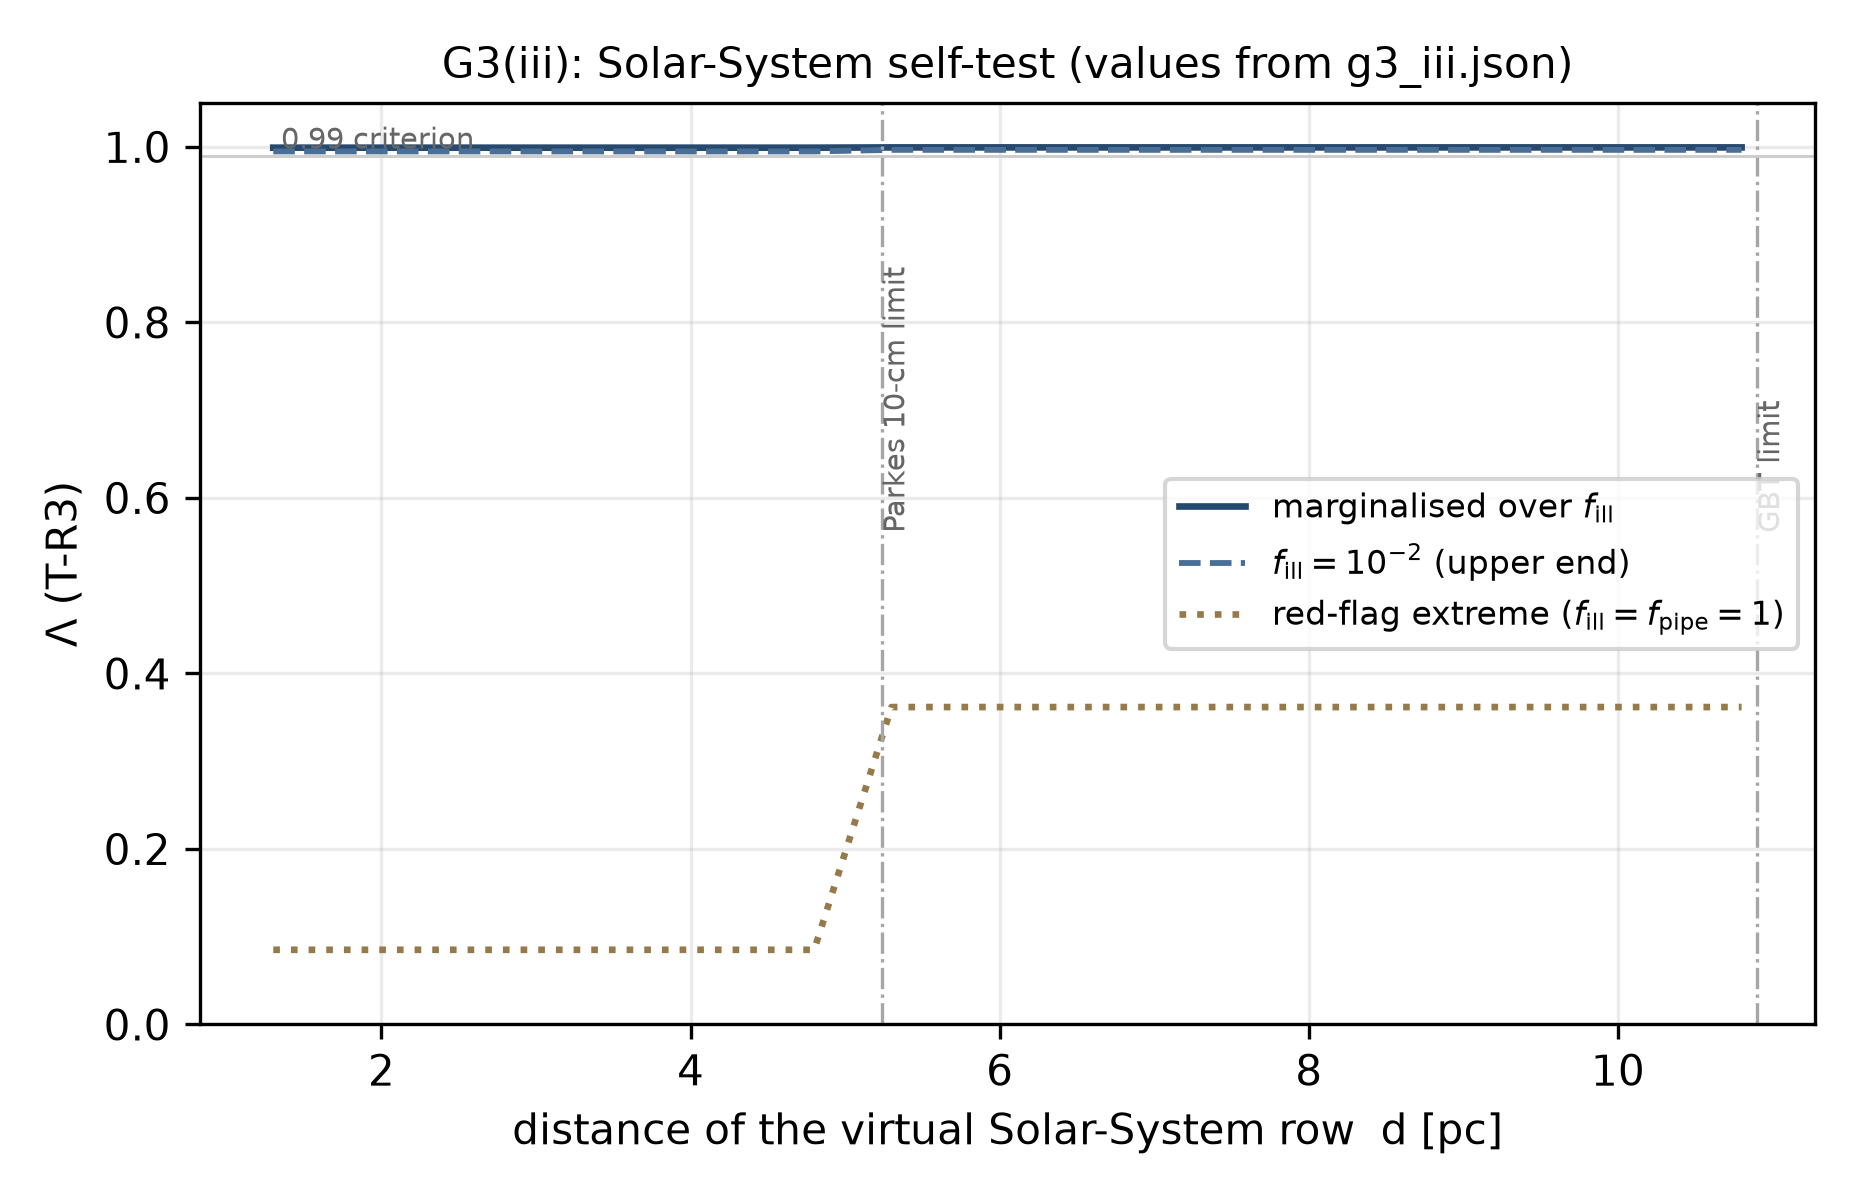
\includegraphics[width=.9\linewidth]{figs/fig1_g3iii_dlambda.png}
\par\smallskip{\small 図 1: G3(iii) 太陽系自己検定の d–\(\Lambda\)。周辺化値・f\_ill = 10\(^{-2}\)(上端)・極限(f\_ill = f\_pipe = 1)の 3 曲線と感度境界(Parkes 5.24 pc、GBT 10.9 pc)。数値は g3\_iii.json の凍結値。再現: python3 scripts/build\_paper\_figs.py}
\end{figure}


\subsection*{4.6 逸脱節(第9条3項): 制度が機能した二つの実例}
\noindent \textbf{裁定 \#3(逸脱: 基準の改訂)}。凍結文書 \S{}5 は G3(i)(b) の \(\leq\)100/200 pc 殻の合格基準を「公刊中心値 \(\pm\)1\%」としていた。再計数 0.0598\% は公刊 0.061\% に対し \(-\)1.89\% で\textbf{不合格}となり、作業を停止した。参謀の原典照会により、WS20 \S{}3 が 50 pc 殻の増分を +42/\(-\)7、EIRP \(\geq\) 10\(^{13}\) W 条件の計数を 1513(+9/\(-\)7)と併記していること、当方の \texttt{b\_rest} 再計数(+42)が原典の +42 と完全一致することが判明した。すなわち、再計数機構は原典と同一に動作しており、中心値の計数手続きは本文から一意復元不能で、不合格の実体は\textbf{凍結時に公刊誤差幅を確認せずに基準を設計した不備}であった。基準を「公刊の明示誤差区間の内側」に改訂(\(\leq\)50 pc の完全一致要件と再計数手続きは不変)し、新基準で合格とした。旧基準での不合格の事実は記録として残す。誤り台帳 E-1(参謀の凍結前検分の不備)・E-2(経緯)。\par\smallskip
\noindent \textbf{裁定 \#4(逸脱ではない: 基準どおりの不合格受理)}。G3(ii) は凍結基準で不合格であり、数字を見た後の適合定義の選択(定義 B)に基づく判定の差し替えは採択せず、T-W1 を降格した。基準の変更を伴わない不合格の受理は、基準改訂(裁定 \#3)と対をなす実例である。\par\smallskip
\noindent 自己申告: 改訂 2 再提出時の追補文の反映漏れ(1 件)、BL 取得対象の集計スクリプトの引き算ミス(取得漏れなし)、裁定ログのパス表記のシェル展開取りこぼし、T-R3 の \(\Lambda\) 下限を 4 桁丸め値の不等号で引用した転記(E-7。厳密値 0.998458 を併記して訂正)、交差計数の補集合ラベルの区分混同(E-8。上界なし 13,984 = 判定不能 13,982 + 感度外 2)。いずれも数値の結論への影響なし(付録 B)。\par\smallskip

\section*{5. Results}

\subsection*{5.1 台帳の概観}
\noindent 空き度上界(\(\varepsilon\) 確定)を持つ星は T-R1 \textbf{1,554}、T-R2 \textbf{1,587}、T-R3 \textbf{159}(d \(\leq\) 10.8 pc)\footnote{\texttt{data/phase2/lambda\_ledger.json}(summary.status\_counts、lambda\_*)。}。観測されたが当該帯で感度外(\(\varepsilon\) = 0、\(\Lambda\) = 1 = 情報なし)の星は T-R1 33、T-R3 1,428。T-R1 の \(\Lambda\) は 0.4266(最小: GBT L + GBT S + GBT S + Parkes 10-cm の 4 観測行、S 帯 2 ポインティング、1 星)/ 0.8000(中央値: GBT S のみ)/ 0.8596(最大: GBT L のみ)で、事後 @\(\pi\) = 10\(^{-2}\) の中央値は 0.0080。T-R3 は \(\Lambda\) = 0.9985–0.9998(4 桁丸め; 最小の厳密値 0.998458)、事後 @\(\pi\) = 10\(^{-2}\) で 0.0100。\(\Lambda\) の値は観測行の被覆構造(受信帯の窓内被覆率 \(\times\) f\_pipe)で決まり、距離にはほとんど依らない(感度閾値をまたぐ星が T-R1 で 33 星のみ。図 2)。\par\smallskip

\begin{figure}[t]\centering
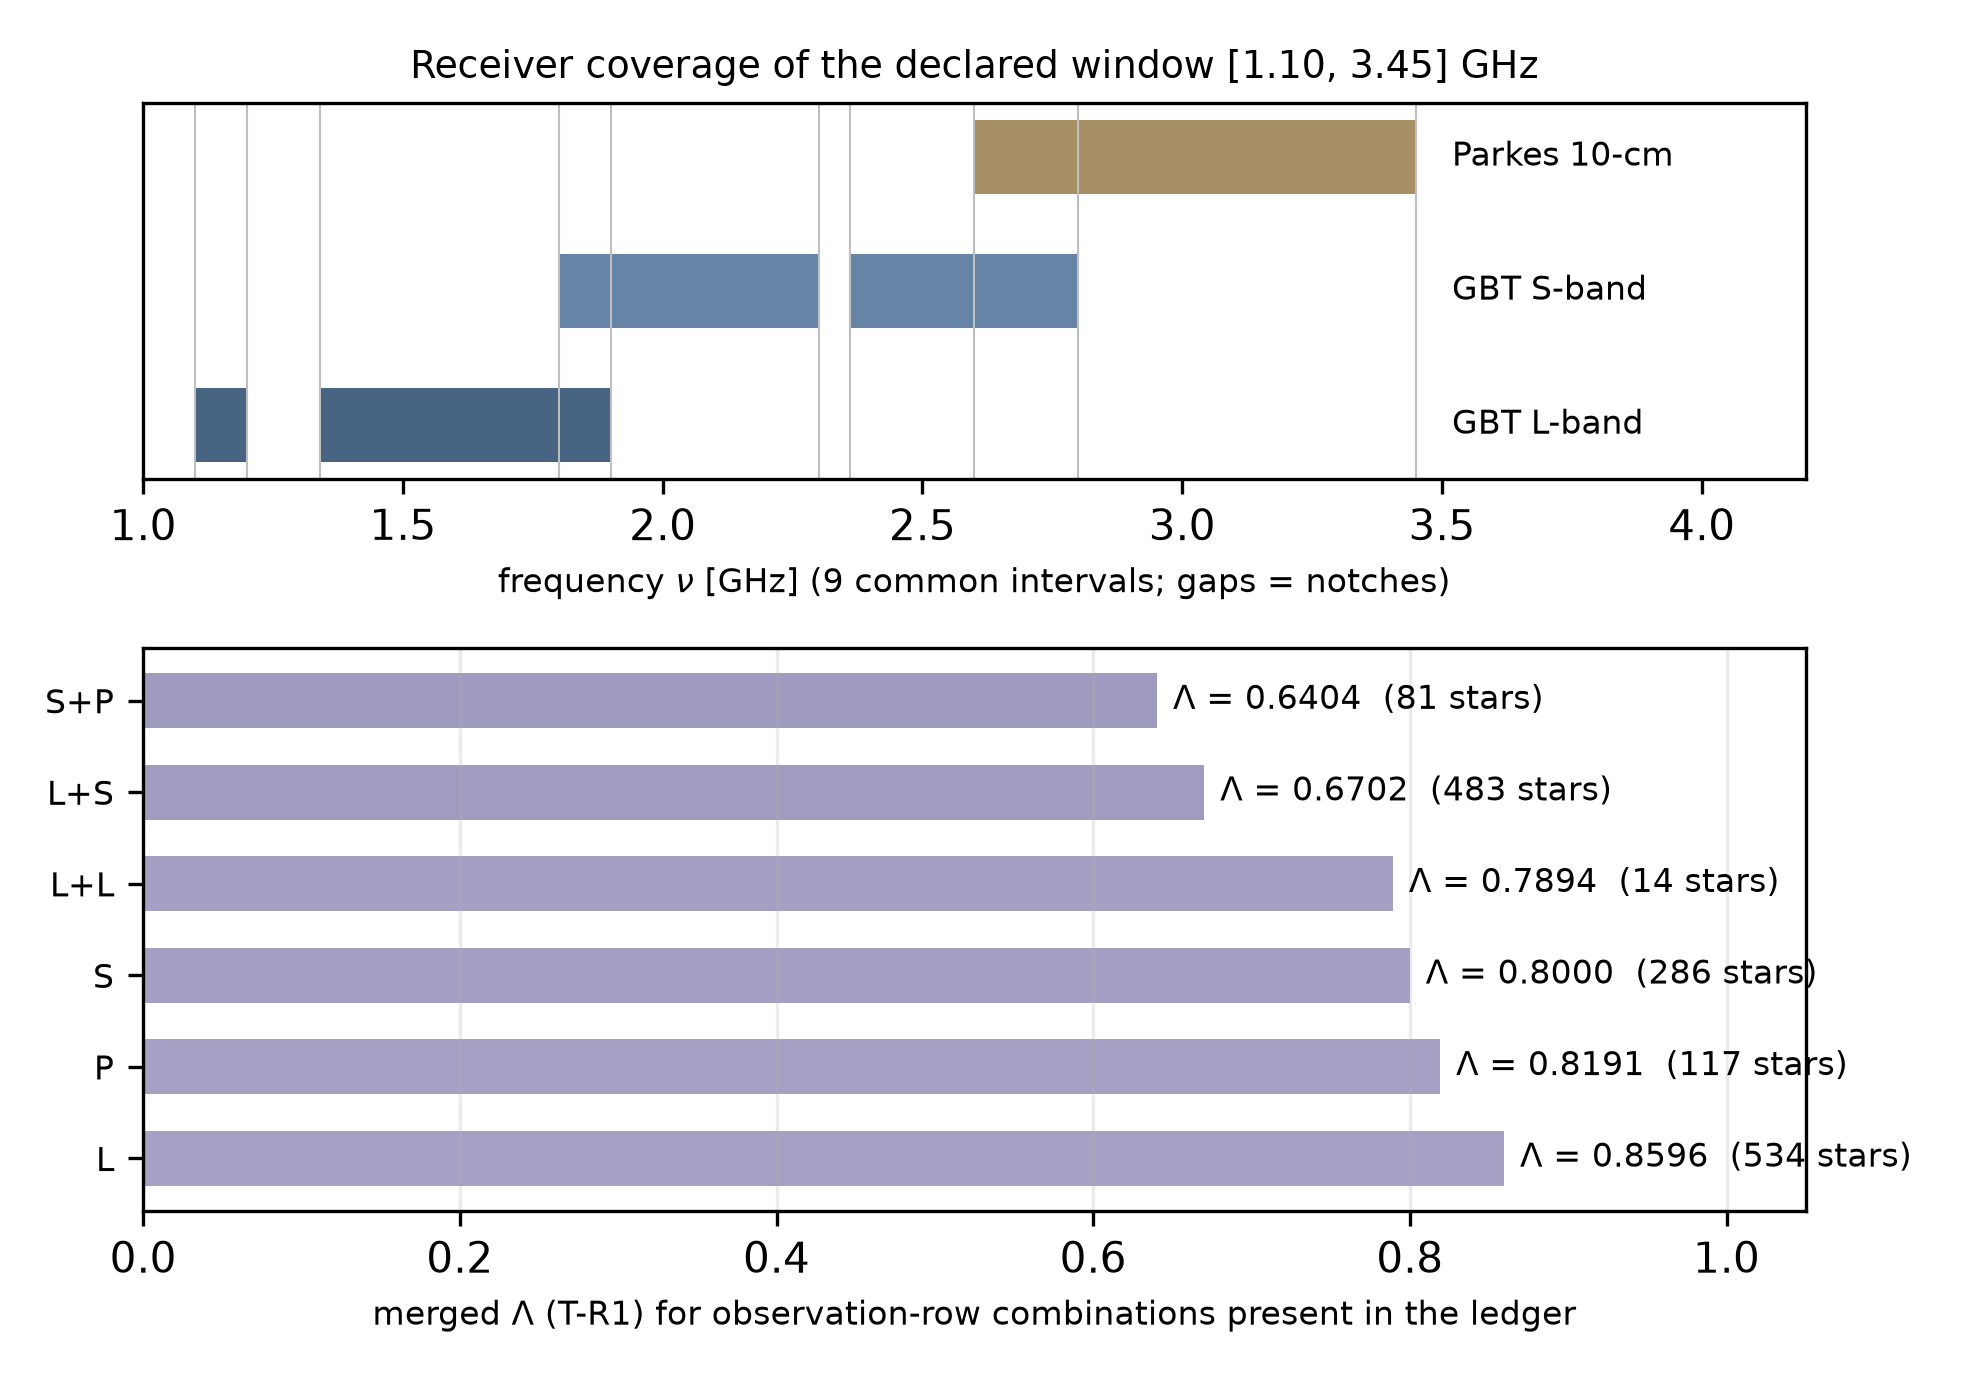
\includegraphics[width=.9\linewidth]{figs/fig2_coverage_lambda.png}
\par\smallskip{\small 図 2: 宣言窓 [1.10, 3.45] GHz の受信帯被覆(上: 9 共通区間とノッチ)と、台帳に実在する観測行組合せごとの併合 \(\Lambda\)(下: T-R1、棒の色は \(\pi\) = 10\(^{-2}\) の事後彩色)。数値は radio\_obs\_v0.json と lambda\_ledger.json の凍結値。再現: python3 scripts/build\_paper\_figs.py}
\end{figure}



\subsection*{5.2 判定不能 99.52\%: 主結果として}
\noindent 母集団 332,571 星のうち、WS20 のいずれのポインティングの視野にも入っていない星は \textbf{330,984(99.52\%)}\footnote{\texttt{data/phase2/lambda\_ledger.json}(summary.status\_counts、lambda\_*)。}。このうち \textbf{1,530 星}は BL 公開アーカイブに観測ファイルがあるが上限が公刊されていない(C/X 帯、または L/S/10-cm で Price+20 非掲載)ため「観測あり・未公刊」として判定不能 (d) に分類した\footnote{\texttt{docs/phase1/00-status.md} \S{}1.3。}。判定不能は空き側にも占有側にも倒さない。この数字は、既存の電波 SETI の不在証拠が太陽近傍 100 pc の星のうち\textbf{どれだけ少ない星にしか及んでいないか}を星単位で示すものであり、Wright+18 のヘイスタック不完備性の星単位版である(図 3)。\par\smallskip

\begin{figure}[t]\centering
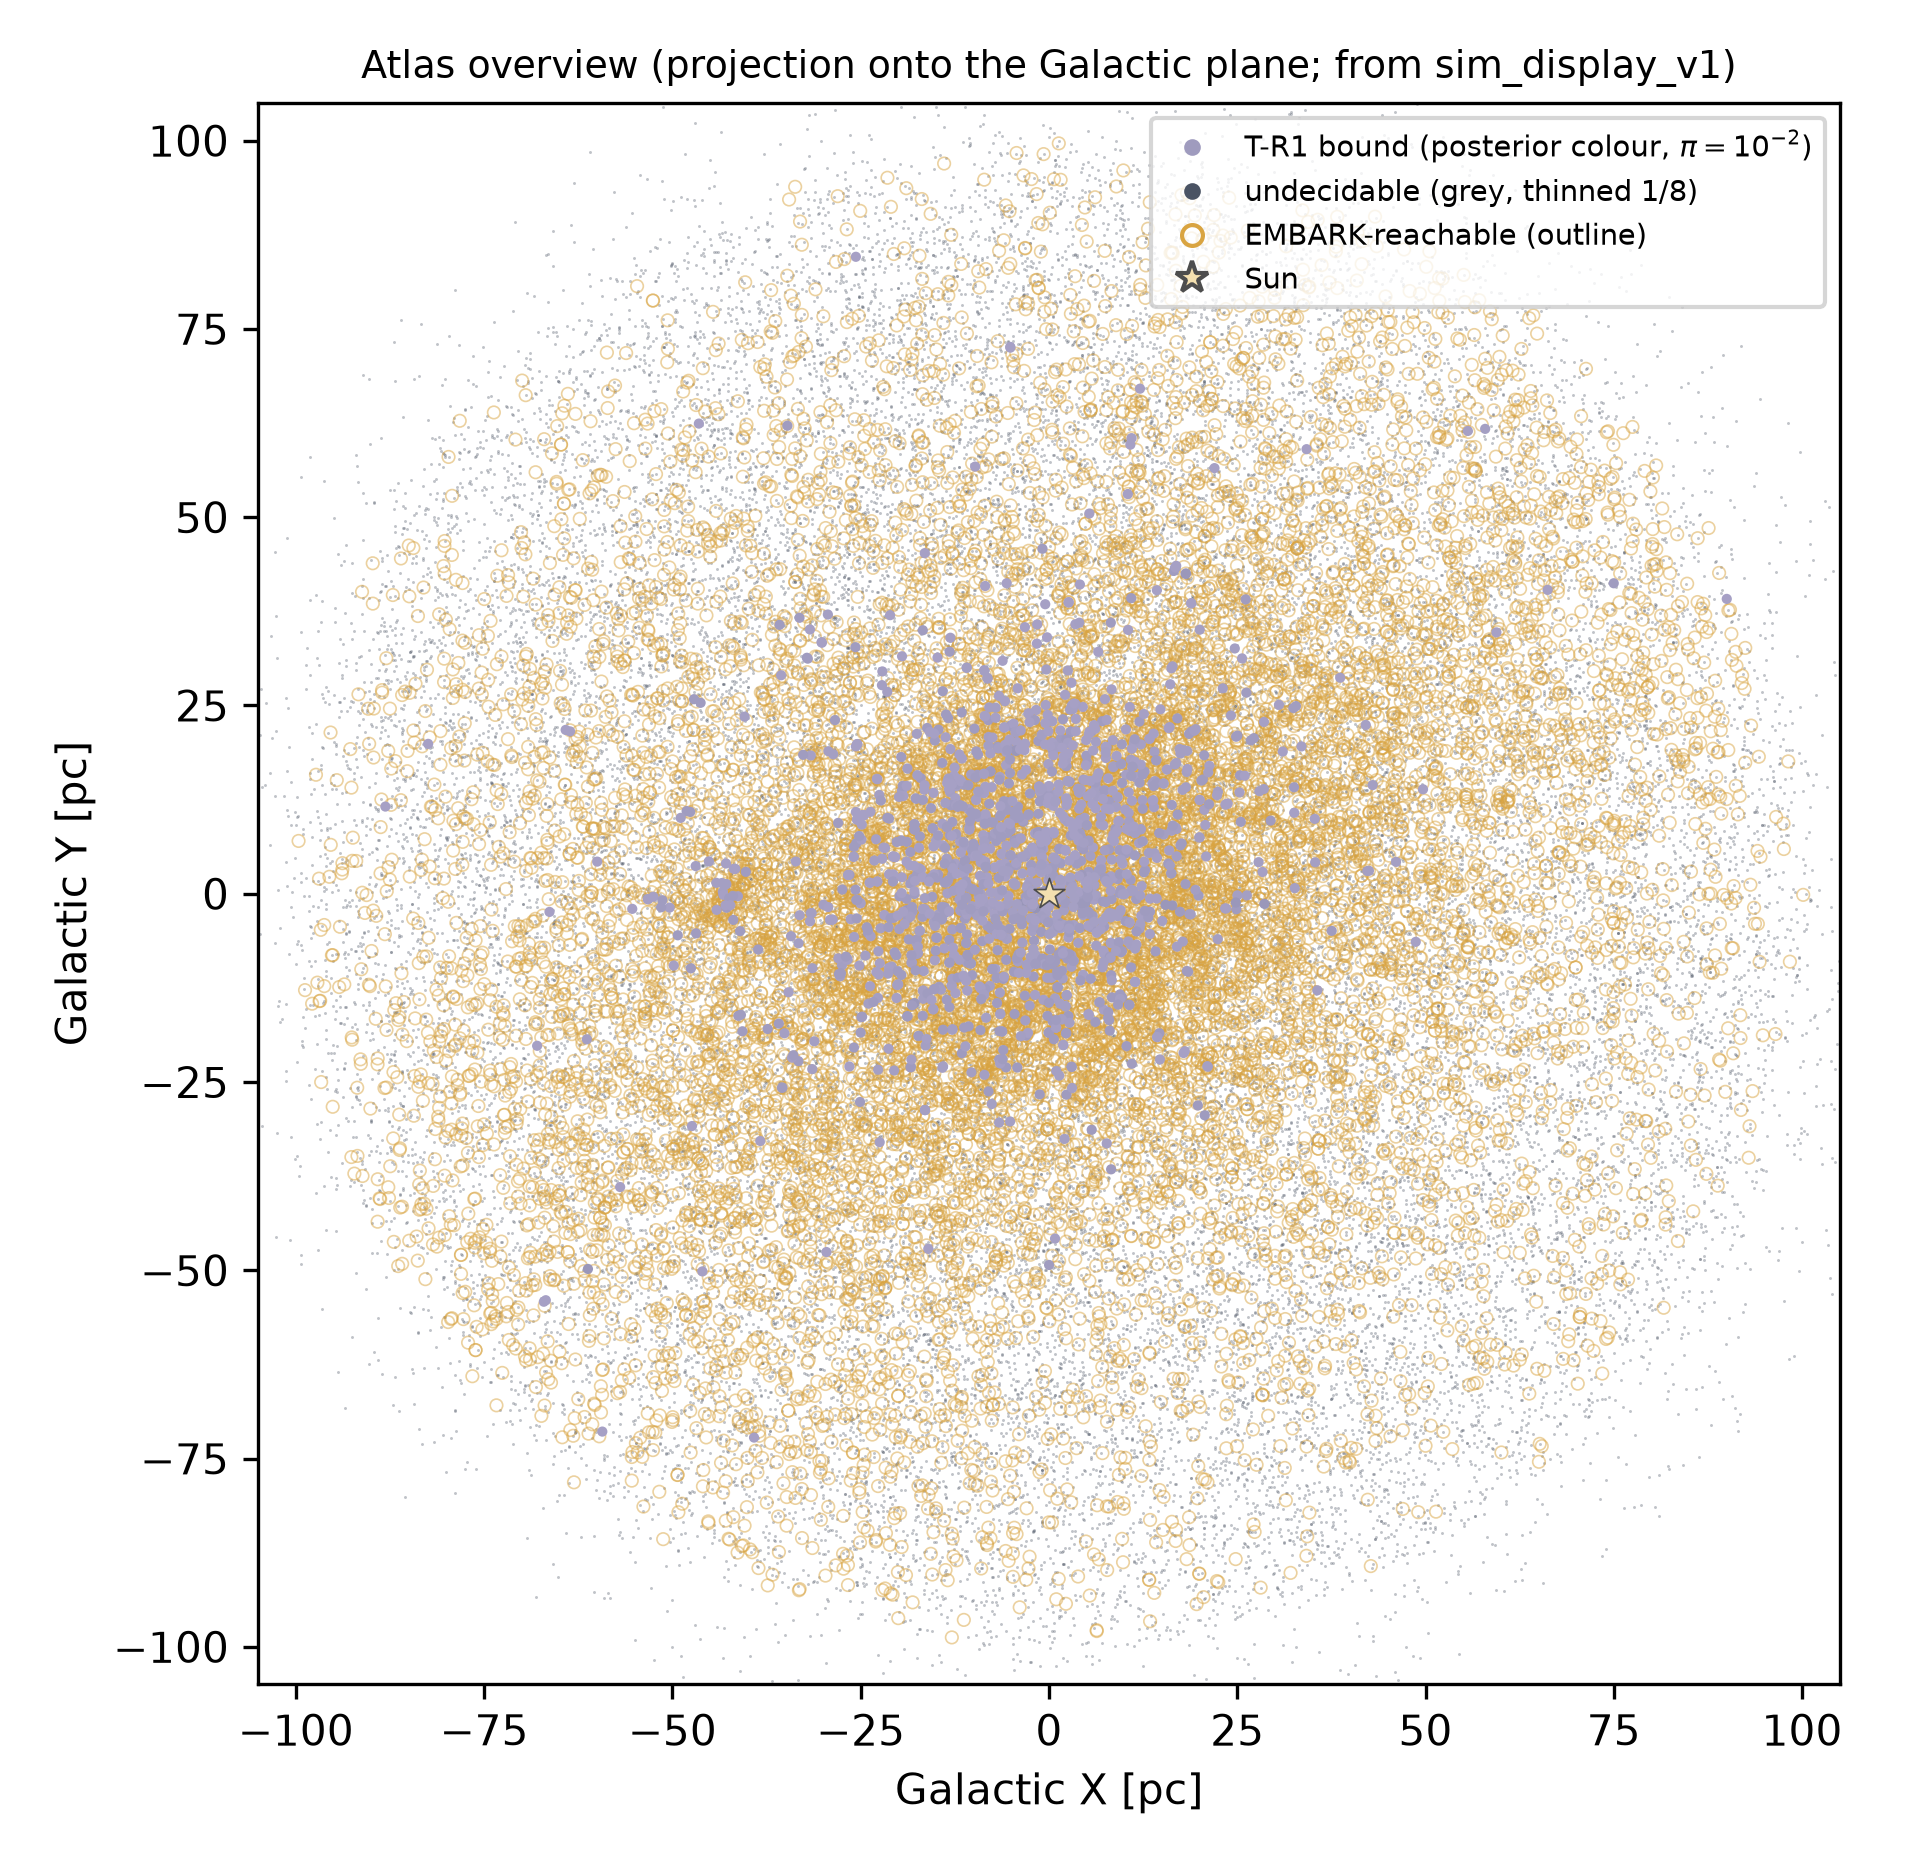
\includegraphics[width=.9\linewidth]{figs/fig3_atlas_overview.png}
\par\smallskip{\small 図 3: アトラス概観(銀河面への投影、sim\_display\_v1 から機械生成)。判定不能星は灰(1/8 間引き)、T-R1 上界あり星は \(\pi\) = 10\(^{-2}\) の事後による中立連続彩色、EMBARK 到達星は輪郭、太陽は星印。シミュレータと同一の配色規律。再現: python3 scripts/build\_paper\_figs.py}
\end{figure}



\subsection*{5.3 上界曲線}
\noindent P(占有 | D, T, \(\pi\)) = expit(logit \(\pi\) + ln \(\Lambda\)) は \(\pi\) の単調関数で、\(\Lambda\) \(\in\) [0.43, 0.86] の電波帯では事後 \(\approx\) \(\pi\) \(\times\) \(\Lambda\)(\(\pi\) \(\ll\) 1)となる。図 4(\(\pi\) 掃引)。\par\smallskip

\begin{figure}[t]\centering
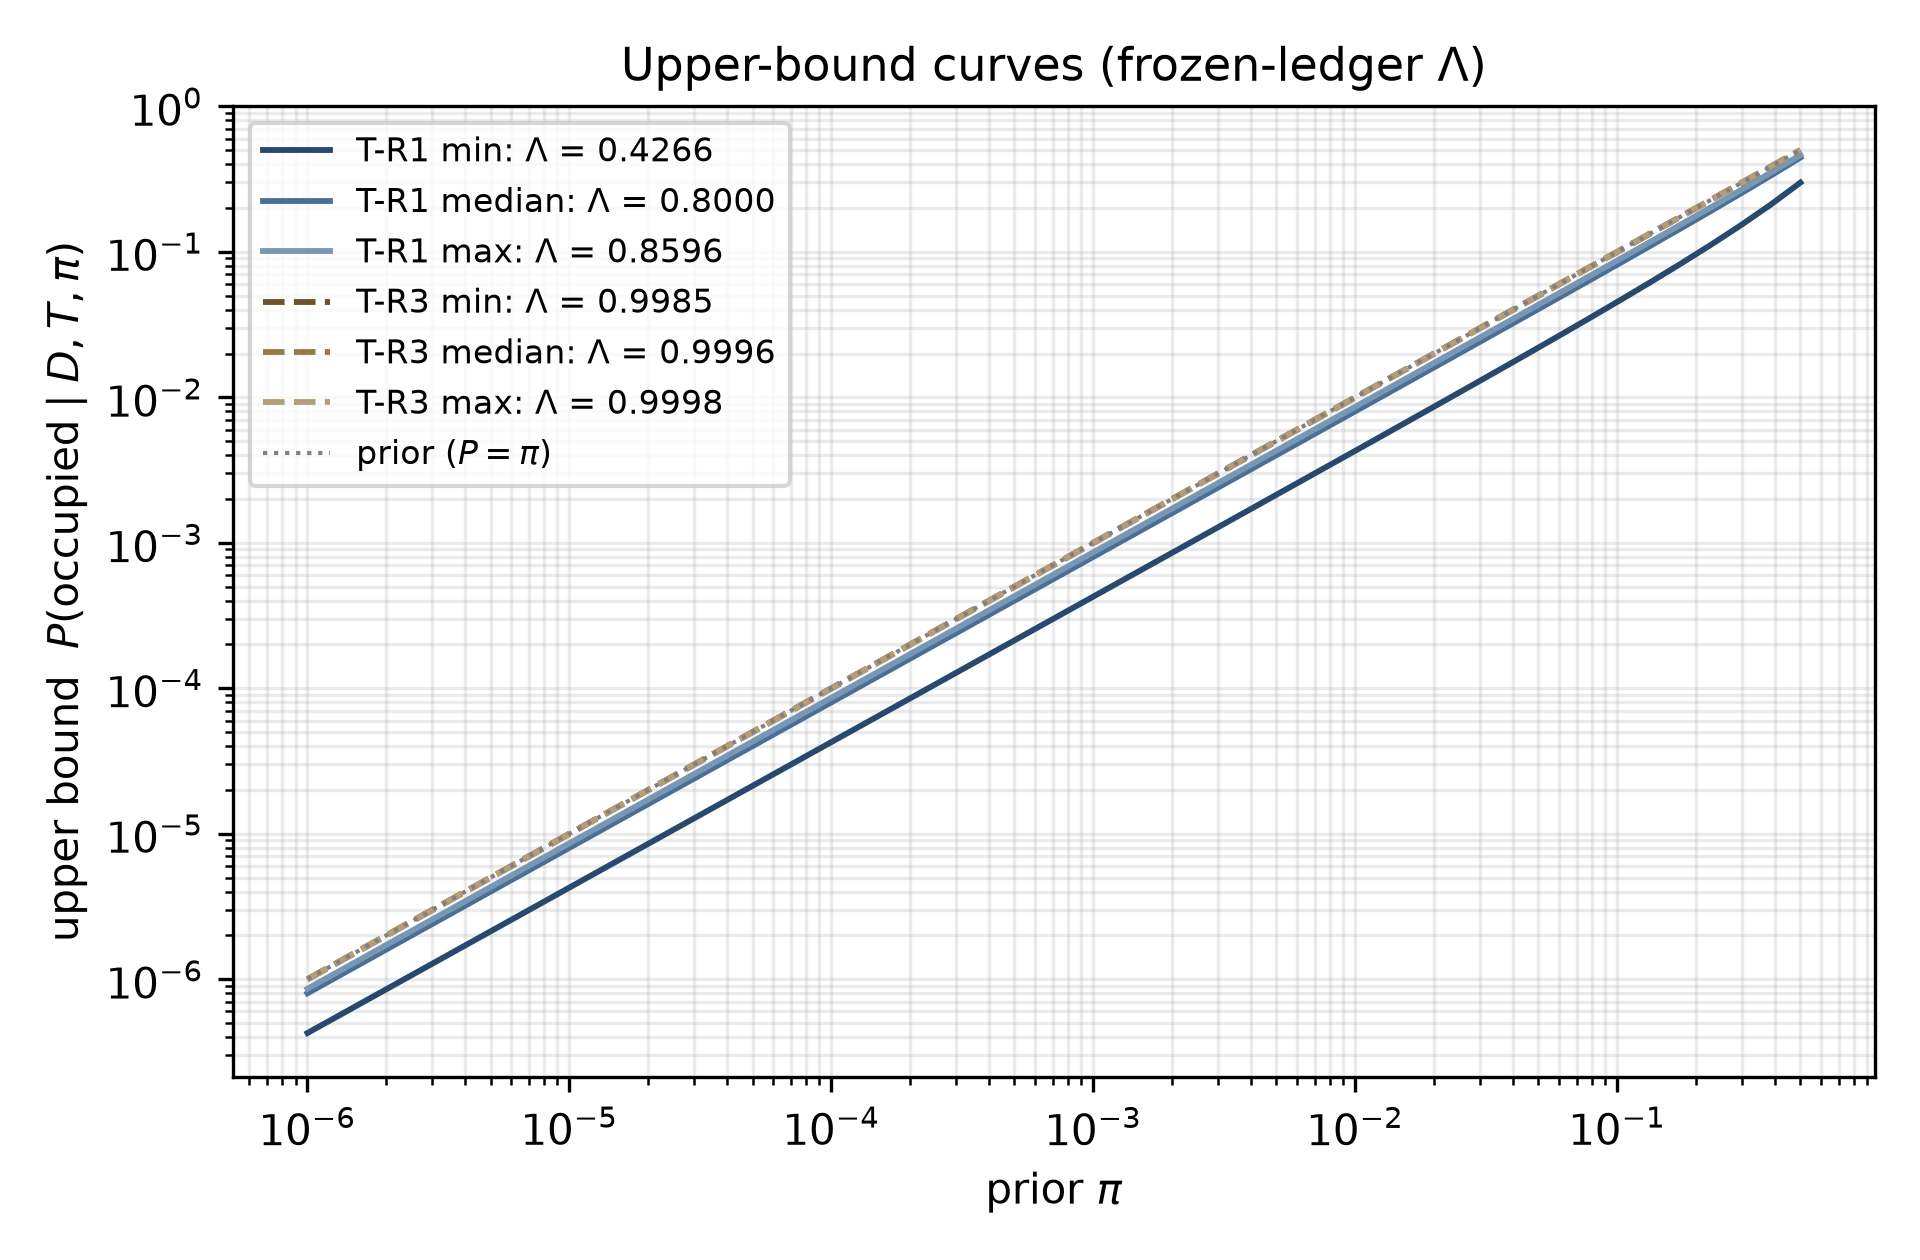
\includegraphics[width=.9\linewidth]{figs/fig4_pi_sweep.png}
\par\smallskip{\small 図 4: \(\pi\) 掃引の上界曲線 P(占有 | D, T, \(\pi\)) = expit(logit \(\pi\) + ln \(\Lambda\))。曲線は凍結台帳の \(\Lambda\)(T-R1 の最小/中央/最大、T-R3 の最小/中央/最大)。点線は事前 P = \(\pi\)。再現: python3 scripts/build\_paper\_figs.py}
\end{figure}
\noindent 「空き度」は曲線であり、単一数値ではない。\par\smallskip

\subsection*{5.4 太陽自己校正}
\noindent 地球級帯 T-R3 では事後 \(\approx\) 事前であり、本アトラスが空き度を語れる技術帯の下限は地球自身で校正される(\S{}4.5)。\par\smallskip

\subsection*{5.5 W1 情報レイヤ(claim=false)}
\noindent GCNS 内蔵の WISE 測光から導いた T-W1 の \(\Lambda\) は、主系列かつ W3/W4 測光を持つ 192,363 星(既超過の検出候補 3,615 星・模型外 54,498 星・測光なし 82,094 星は判定不能)のうち、\(\gamma\) = 0.1 で \(\Lambda\) < 1(\(\varepsilon\) > 0)の星が 191,237(その大半は \(\Lambda\) = 0 = 全 T\_DS 区間で検出されたはず)、感度外 \(\Lambda\) = 1 が 1,126 である\footnote{\texttt{data/phase2/lambda\_ledger.json}(lambda\_W1\_g0.1)。\(\Lambda\) < 1 の計数には \(\Lambda\) = 0 の星を含む。}。これは物理的に正しい: 太陽を 10 pc に置いた 12 \(\mu\)m の光球流束 1.9 Jy に対し、\(\gamma\) = 0.1・300 K の部分ダイソン球は 90 Jy を放つ。しかしこの導出は G3(ii) のアンカー不合格により主張の地位を持たず、v1 では情報レイヤ(既定オフ、「アンカー未確立」バッジ)として提供する。\par\smallskip


\section*{6. Three-axis atlas}

\subsection*{6.1 結合率}
\noindent 到達可能性は EMBARK reachability atlas v1(37,498 星)を DR3 source\_id で結合した: GCNS 内在 \textbf{14,799}(4.45\%)、残り 22,699 星は 100 pc 超で母集団外(注記のみ)、GCNS 側の 317,772 星(95.55\%)は到達可能性\textbf{判定不能}\footnote{\texttt{data/phase4/atlas\_v1\_summary.json}。}。定住資源性は GCNS 内蔵量(M\_G、BP\(-\)RP、WDprob)、Mamajek 表の色\(\rightarrow\)型区分、NASA Exoplanet Archive(1,037 ホスト・1,545 惑星)、HWC(居住可能候補 70 行中 45 行・35 ホスト)を結合した。三軸とも既存カタログの値をそのまま用い、再計算は行っていない。\par\smallskip


\subsection*{6.2 交差計数(合成なし)}
{\footnotesize\setlength{\tabcolsep}{3.5pt}\begin{center}\begin{tabular}{ll}
条件 & 星数 \\
\hline
EMBARK 会合到達(いずれかのセル)\(\wedge\) T-R1 上界あり & \textbf{815} \\
同 \(\wedge\) T-R3 上界あり & 108 \\
EMBARK 同行到達 \(\wedge\) T-R1 上界あり & 311(同行到達 2,339 のうち) \\
T-R1 上界あり(1,554)のうち EMBARK 外 & 739 \\
T-R1 上界あり \(\wedge\) S1(FGK 主系列)/ S2(主系列全型) & 633 / 1,406 \\
T-R1 上界あり \(\wedge\) 既知惑星ホスト & 136 \\
\end{tabular}\end{center}}
\noindent 会計: 1,554 = 815 + 739。\(\Lambda\) の分布は EMBARK セルに依らず同じ(空き度は観測行の被覆構造で決まり、到達性と独立)。各セルの条件節は台帳 JSON に付す。\par\smallskip

\subsection*{6.3 定住資源性スライダー}
\noindent S1 狭義(FGK 主系列、Mamajek 区分 F0–K5)43,119 星 / S2 主系列全型 283,526 星 / S3 資源的広義(全恒星)332,571 星。スライダーは表示時の星集合の関数であり判定基準ではなく、空き度・到達可能性の値に影響しない。狭義ハビタビリティ(液体の水・温度)は判定基準にしない。\par\smallskip

\subsection*{6.4 HWC 照合表(合成ではない)}
\noindent HWC 居住可能候補ホストのうち T-R1 上界を持つものは 16(例: Proxima Cen b のホスト \(\Lambda\) = 0.819、EMBARK 到達; Ross 128 b のホスト \(\Lambda\) = 0.860、EMBARK 外)。TRAPPIST-1、LHS 1140、TOI-700 等 19 ホストは電波視野外で空き度判定不能。居住可能候補であることと空き度上界は独立に取得された量であり、本表は照合のみで合成しない。\par\smallskip

\section*{7. Discussion}

\subsection*{7.1 解釈の範囲と限界(Interpretation and scope)}
\noindent 本稿の結果は次の四点の範囲でのみ意味を持つ。第一に、本台帳は測量であって証明ではない。不在の証拠は限定的であり、占有の不在を証明しない。第二に、空き度上界は入植許可証ではない。本成果物から占有の不在や入植の正当性を推論することはできない。第三に、HWC 照合表は合成ではない。居住可能候補と空き度上界を掛け合わせた量は本稿のどこにも存在しない。第四に、1/N と星単位事後は別量であり、数値の近さ(\S{}4.3(c))は偶然である。同じ理由から、本稿の値は条件節(技術帯・サーベイ集合・\(\pi\))を離れては意味を持たない。単一数値や順位への圧縮、三軸の積・加重和、判定不能星を空き側に数えること、本成果物を入植・接触・送信の正当化に用いることは、いずれも本手法の範囲外の使用である。W1 情報レイヤはアンカー未確立であり、空き度の主張には用いない。\par\smallskip

\subsection*{7.2 限界と展望(Limitations and outlook)}
\begin{itemize}\setlength{\itemsep}{1pt}
\item \textbf{未公刊観測}: BL 公開アーカイブには GCNS 星 1,530 の未公刊観測(C/X 帯等)があり、上限の公刊により判定不能 (d) から可判定へ移りうる。UWL・光学レーザー・遷移現象は拡張区画。
\item \textbf{独立性仮定}: f\_pipe の観測間独立は Price+20 と同一前提だが、感度枠(U[0.3, 0.8])の外に相関の効果が残りうる。
\item \textbf{W1 の再アンカー}: 受動的(Hephaistos 星単位表の公開、または DR4 v1.1 での独立アンカー)。
\item \textbf{DR4 合流(2026-12-02)}: 恒星基盤を DR4 に差し替え、\(\varepsilon\) 台帳は距離更新分のみ再計算する v1.1 を出す(EMBARK v1.1 と同期)。
\item \textbf{母集団の地平線}: GCNS \(\leq\)100 pc であり、WS20 の 288,315 星の大半(100 pc 超)は本アトラスの母集団外である。
\end{itemize}

\section*{付録 A: \(\varepsilon\) 因子表・受信帯被覆・共通 \(\nu\) グリッド}
\noindent 事前登録 (b)(\url{doi:10.5281/zenodo.22067884})\S{}2 の転記: EIRP50、ビーム応答、受信帯被覆(L [1.10,1.20]\(\cup\)[1.34,1.90]、S [1.80,2.30]\(\cup\)[2.36,2.80]、P [2.60,3.45] GHz)、共通 \(\nu\) グリッド境界 \{1.10, 1.20, 1.34, 1.80, 1.90, 2.30, 2.36, 2.60, 2.80, 3.45\}、f\_pipe 0.5、f\_ill 格子 13 点、T\_DS 20 区間、k = 3、S/N \(\geq\) 3.5、主系列選択式、Mamajek 表 sha256 1de2edee\ldots{}、WISE 零点。\par\smallskip

\section*{付録 B: Method record and AI disclosure}
\noindent 三役: 人間(前田幸枝)= 方向設定・ゲート裁定・全分岐の最終決定 / チャット Claude = 参謀・独立検算(G2 第二経路)・文献照合 / Claude Code(Fable 5)= 実行。運用記録: 裁定 8 件(\#1 技術帯集合 A–F、\#2 事前登録 (b) 修正、\#3 逸脱・基準改訂、\#4 不合格受理・降格、\#5 付議 7 件、\#6 目次承認、\#7 報告 (2) 条件付き承認、\#8 公開前の体裁・文体)、停止 2 回(G3(i)(b)、G3(ii)。いずれも正しく停止し裁定で再開)、逸脱 1、不合格 1、自己申告 5(追補反映漏れ・BL 集計・ログ表記・E-7・E-8)。誤り台帳 r1(E-1〜E-8)。本内部検証は人間による査読の代替ではない。\par\smallskip

\section*{付録 C: 判定不能会計(三軸)}
{\footnotesize\setlength{\tabcolsep}{3.5pt}\begin{center}\begin{tabular}{lll}
軸 & 判定不能 & 率 \\
\hline
空き度(電波 3 帯、視野外) & 330,984 & 99.52\% \\
空き度(W1) & 拡張区画(情報レイヤ) & 該当なし \\
到達可能性(EMBARK 外) & 317,772 & 95.55\% \\
定住資源性(測光なし) & 8,261 & 2.48\% \\
\end{tabular}\end{center}}

\section*{付録 D: Reproducibility and data release}
\noindent 再生成: \texttt{python3 src/vacancy/build\_ledger.py}(3 s)/ 図 1–4: \texttt{python3 scripts/build\_paper\_figs.py}\(\rightarrow\) \texttt{scripts/export\_g2.py} \(\rightarrow\) \texttt{python3 src/vacancy/aggregate.py}(\(\approx\)10 分)\(\rightarrow\) \texttt{scripts/g3\_i\_ws20\_price.py} / \texttt{g3\_ii\_hephaistos.py} / \texttt{g3\_iii\_solar\_selftest.py} \(\rightarrow\) \texttt{python3 src/vacancy/build\_atlas.py}。単体テスト \texttt{python3 -m unittest tests.test\_epsilon}(14 件)。公開物: \(\varepsilon\) 台帳(\texttt{ledger\_v0.json}、式版 eps-v0.2)、\(\Lambda\) 台帳(\texttt{lambda\_ledger.json})、三軸アトラス(\texttt{atlas\_v1.json})、電波観測行来歴(\texttt{radio\_obs\_v0.json})、G1/G2/G3 レポート、NEA/HWC 凍結コピー、全スクリプト、誤り台帳 r1、sha256 マニフェスト(\texttt{MANIFEST.json})。事前登録 (a) コミット 10a01e710854b69344651ed6ba016ab303c9d124、(b) \url{doi:10.5281/zenodo.22067884}。\par\smallskip

\section*{謝辞}
\noindent This work has made use of data from the European Space Agency (ESA) mission Gaia (\url{https://www.cosmos.esa.int/gaia}), processed by the Gaia Data Processing and Analysis Consortium (DPAC, \url{https://www.cosmos.esa.int/web/gaia/dpac/consortium}). Funding for the DPAC has been provided by national institutions, in particular the institutions participating in the Gaia Multilateral Agreement. This research has made use of the NASA Exoplanet Archive, which is operated by the California Institute of Technology, under contract with the National Aeronautics and Space Administration under the Exoplanet Exploration Program. This research has made use of the VizieR catalogue access tool, CDS, Strasbourg, France (DOI: 10.26093/cds/vizier). The Habitable Worlds Catalog is maintained by the Planetary Habitability Laboratory @ UPR Arecibo. Breakthrough Listen 公開データアーカイブ(seti.berkeley.edu/opendata)の観測メタデータを使用した。\par\smallskip

\section*{参考文献}

\noindent [1] Price D. C. et al. 2020, AJ 159, 86.\par\smallskip
\noindent [2] Wlodarczyk-Sroka B. S., Garrett M. A., Siemion A. P. V. 2020, MNRAS 498, 5720.\par\smallskip
\noindent [3] Enriquez J. E. et al. 2017, ApJ 849, 104.\par\smallskip
\noindent [4] Isaacson H. et al. 2017, PASP 129, 054501.\par\smallskip
\noindent [5] Lebofsky M. et al. 2019, PASP 131, 124505.\par\smallskip
\noindent [6] Suazo M. et al. 2022, MNRAS 512, 2988.\par\smallskip
\noindent [7] Suazo M. et al. 2024, MNRAS 531, 695.\par\smallskip
\noindent [8] Wright J. T. et al. 2014a, ApJ 792, 26.\par\smallskip
\noindent [9] Wright J. T. et al. 2014b, ApJ 792, 27.\par\smallskip
\noindent [10] Griffith R. L. et al. 2015, ApJS 217, 25.\par\smallskip
\noindent [11] Wright J. T., Kanodia S., Lubar E. 2018, AJ 156, 260.\par\smallskip
\noindent [12] Grimaldi C. 2017, Sci. Rep. 7, 46273.\par\smallskip
\noindent [13] Gaia Collaboration, Smart R. L. et al. 2021, A\&A 649, A6.\par\smallskip
\noindent [14] Gaia Collaboration 2016, A\&A 595, A1.\par\smallskip
\noindent [15] Gaia Collaboration 2021, A\&A 649, A1.\par\smallskip
\noindent [16] Gaia Collaboration 2023, A\&A 674, A1.\par\smallskip
\noindent [17] Brandt T. D. 2021, ApJS 254, 42.\par\smallskip
\noindent [18] Bailer-Jones C. A. L. et al. 2018, AJ 156, 58.\par\smallskip
\noindent [19] Pecaut M. J., Mamajek E. E. 2013, ApJS 208, 9.\par\smallskip
\noindent [20] Wright E. L. et al. 2010, AJ 140, 1868.\par\smallskip
\noindent [21] Cutri R. M. et al. 2014, VizieR On-line Data Catalog II/328.\par\smallskip
\noindent [22] Marocco F. et al. 2021, ApJS 253, 8.\par\smallskip
\noindent [23] Jarrett T. H. et al. 2011, ApJ 735, 112.\par\smallskip
\noindent [24] Sullivan W. T., Brown S., Wetherill C. 1978, Science 199, 377.\par\smallskip
\noindent [25] Saide R. C. et al. 2023, MNRAS 522, 2393.\par\smallskip
\noindent [26] Sheikh S. Z. et al. 2019, ApJ 884, 14.\par\smallskip
\noindent [27] NASA Exoplanet Archive, Planetary Systems Composite Parameters, \url{doi:10.26133/NEA12}(2026-08-23 取得).\par\smallskip
\noindent [28] Habitable Worlds Catalog, PHL @ UPR Arecibo(2026-08-23 取得).\par\smallskip
\noindent [29] Maeda Y. 2026a, Zenodo, \url{doi:10.5281/zenodo.22067884}(事前登録 (b)).\par\smallskip
\noindent [30] Maeda Y. 2026b, WAKE, Zenodo, \url{doi:10.5281/zenodo.21966305.}\par\smallskip
\noindent [31] Maeda Y. 2026c, EMBARK, Zenodo, \url{doi:10.5281/zenodo.22059576.}\par\smallskip
\end{document}
